\chapter{New Concepts}
\label{chap:new_concepts}
Accurately interpreting complex diagrams is essential for many analytical and computational tasks. In the context of \acrshort{xgee}, this involves breaking down screenshots into meaningful components through tokenization. This process, however, depends on the robustness and reliability of the underlying algorithms. This chapter aims to build upon the original algorithms, improving detection accuracy, versatility and ensuring stability.

\section{Edge Detection}
\label{sec:edge_detection}
Edges represent connections between vertices, inputs and outputs. Detecting edges accurately requires an approach that can identify individual line segments and how they connect to form complex chains. This section introduces a robust edge detection pipeline leveraging multiple computer vision techniques to reliably identify edges across a wide variety of block diagrams within \acrshort{xgee}.

\begin{wrapfigure}{R}{0.4\textwidth}
    \centering
    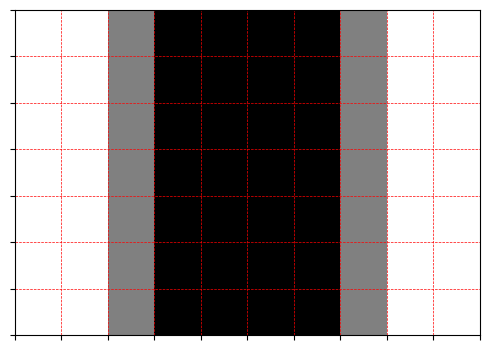
\includegraphics[width=\linewidth]{pictures/kernel_ver.png}
    \caption{kernel used for vertical edge detection, rotated by 90\textdegree\ to generate the horizontal kernel.}
    \label{fig:kernel_ver}
\end{wrapfigure}
Since there are only vertical and horizontal edges within \acrshort{xgee}, two kernels are used to find all pixels containing part of a vertical or horizontal edge. The \textit{filter2D()} function places the kernel anchor (usually the top left value of the kernel) on top of a pixel, with the rest of the kernel overlapping the corresponding local pixels. The kernel values are then multiplied by the corresponding pixel values underneath and added together. The result is saved and placed on the location of the anchor. The vertical kernel in \autoref{fig:kernel_ver} is rotated by 90$^{\circ}$ to generate the horizontal kernel.\\
The same process can be expressed using \autoref{eq:filter2D}, where $H$ is the resulting matrix, $I$ is the original image and $K$ is the used kernel, with $x$, $y$, $i$ and $j$ representing individual pixels within the image $I$ and the kernel $K$. This process is repeated for every pixel and, depending on the structure of the kernel, it can also be used to blur or sharpen an image \cite{opencv_filter2d_2024}.\\
Each value in the processed image is normalized to an 8-bit integer between 0 and 255. This allows the data to be visualized as a gray scale image as seen in \autoref{fig:filter2d} and processed further using \acrshort{opencv}'s \textit{thresholding()} function, seen in \autoref{fig:threshold}, to extract the detected pixels.\\
As illustrated in \autoref{fig:comparison_filter}, ports and letters are sometimes misidentified as edges. Additionally, intersections of edges as well as points where horizontal and vertical edges meet are not immediately detected. These challenging areas will be processed individually in a later step in the edge detection pipeline. Apart from these specific cases, the method effectively extracts all pixels corresponding to vertical and horizontal edges, provided their widths match those of the used kernels.
\begin{equation}
\label{eq:filter2D}
    H(x, y) = \sum_{i=0}^{M_i-1} \sum_{j=0}^{M_j-1} I(x + i - a_i,y + j - a_j)K(i, j)
\end{equation}

\newpage

\begin{figure}[htb]
    \centering
    \includegraphics[width=1\linewidth]{pictures/filter2D.png}
    \caption{Filter2D function results for the horizontal (left) and vertical (right) kernel before thresholding. \textit{edge-like} pixels are colored yellow, while \textit{non-edge-like} pixels are colored purple.}
    \label{fig:filter2d}

    \centering
    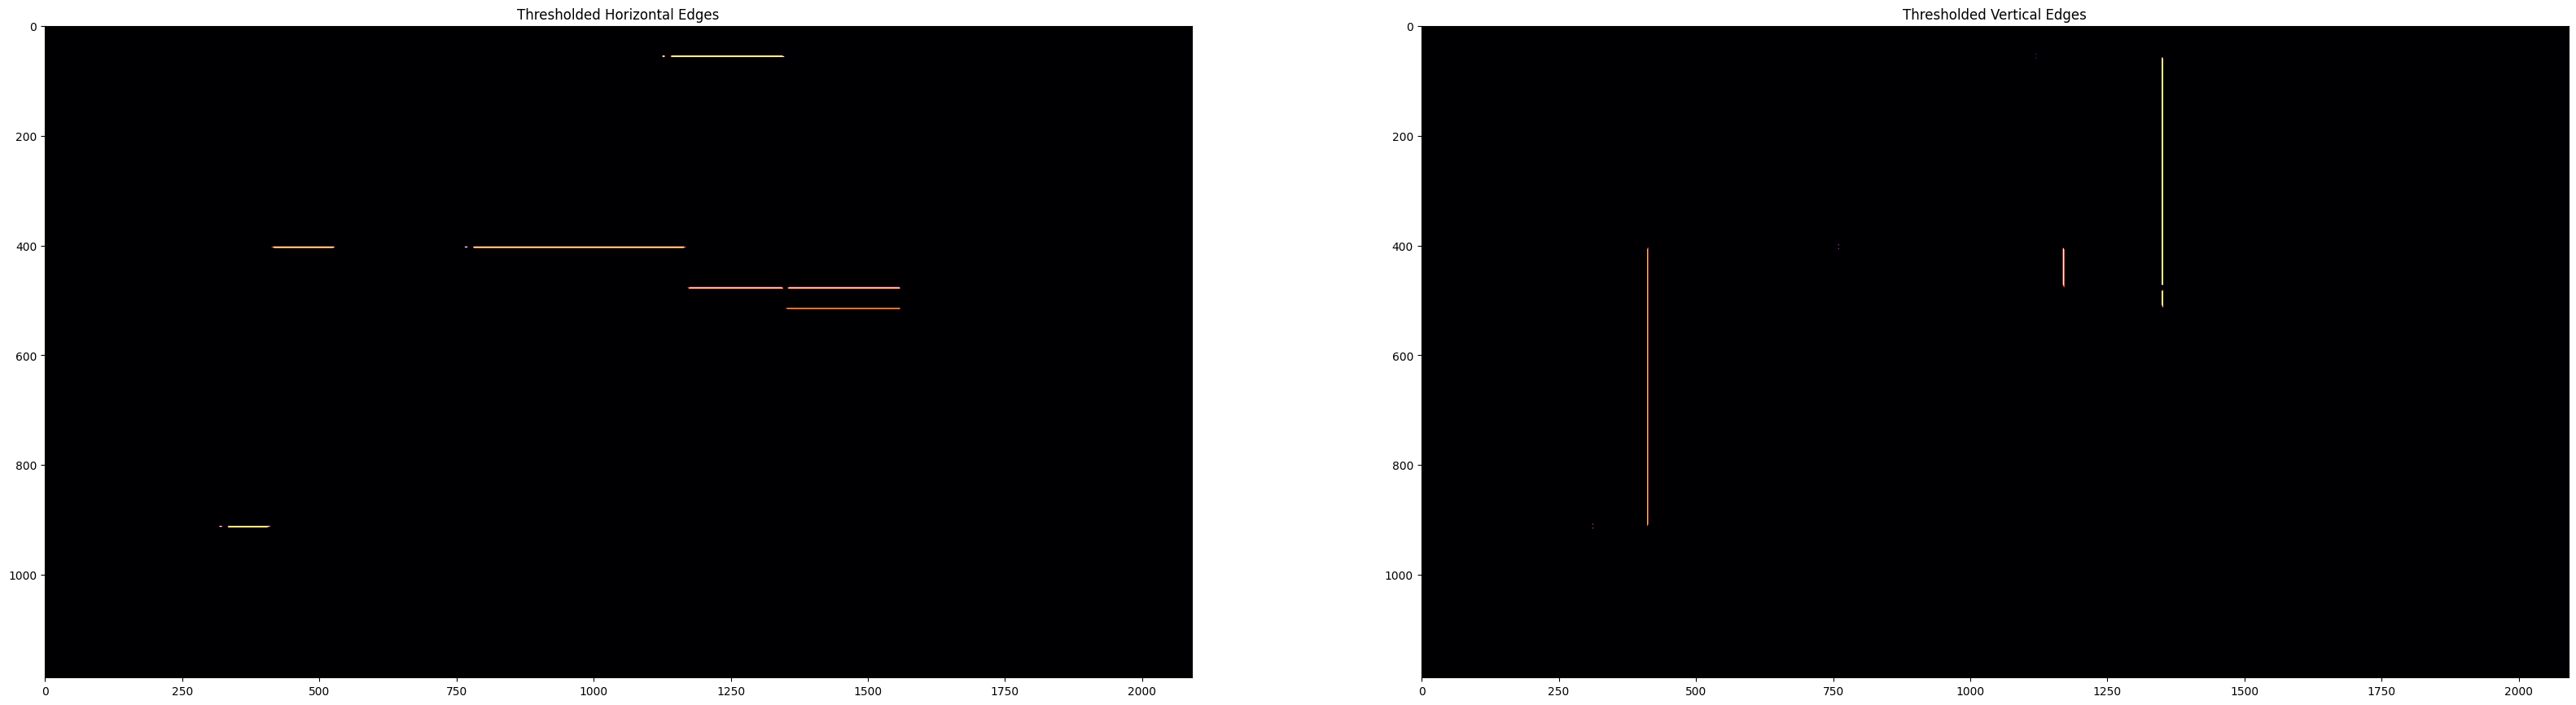
\includegraphics[width=1\linewidth]{pictures/threshold.png}
    \caption{Thresholded filter2D function results. \textit{Edge-like} pixels are now isolated.}
    \label{fig:threshold}
\end{figure}
For easier subsequent processing and data storage, the thresholded pixels seen in \autoref{fig:threshold} are converted to line segments consisting of start- and endpoints. This is achieved through two of \acrshort{opencv}'s built-in functions:\\
\textit{findContours()}, which retrieves contours from a binary image using an algorithm introduced by Satoshi Suzuki and others in \cite{suzuki_1985}. In this context, it is used to group nearby pixels and represent them as narrow polygons.\\
\textit{approxPolyDP()}, which approximates a curve or a polygon with another curve or polygon with less vertices using an algorithm introduced by David H Douglas and Thomas K Peucker in their paper: \cite{douglas_peucker_1973}. This function is used to simplify the contours found by \textit{findContours()} into line segments.
\begin{figure}[ht]
  \centering
  \begin{minipage}[b]{0.45\textwidth}
    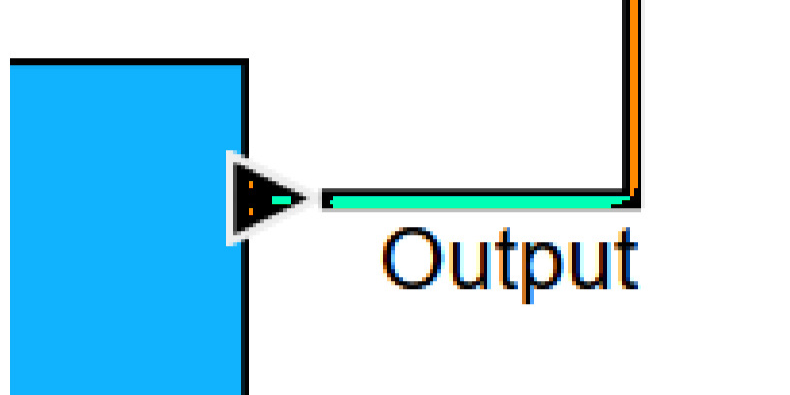
\includegraphics[width=\textwidth]{pictures/thresh_zoom.png}
  \end{minipage}
  \hfill
  \begin{minipage}[b]{0.45\textwidth}
    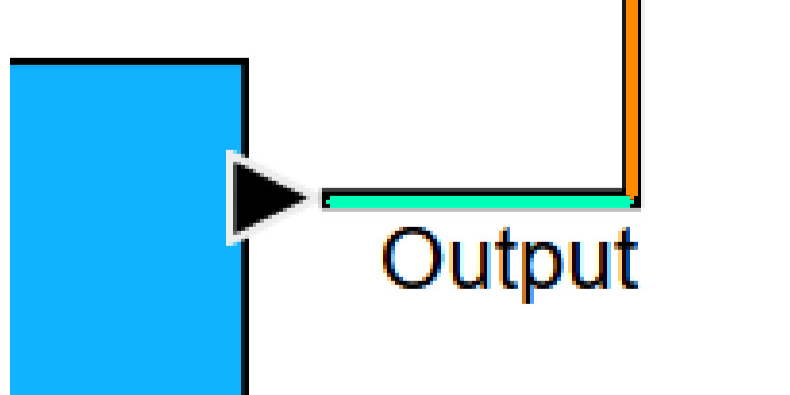
\includegraphics[width=\textwidth]{pictures/line_segments_zoom.png}
  \end{minipage}
  \caption{Comparison of detected pixels and line segments around an output before and after filtering short segments.}
  \label{fig:comparison_filter}
\end{figure}
\begin{figure}[ht]
    \centering
    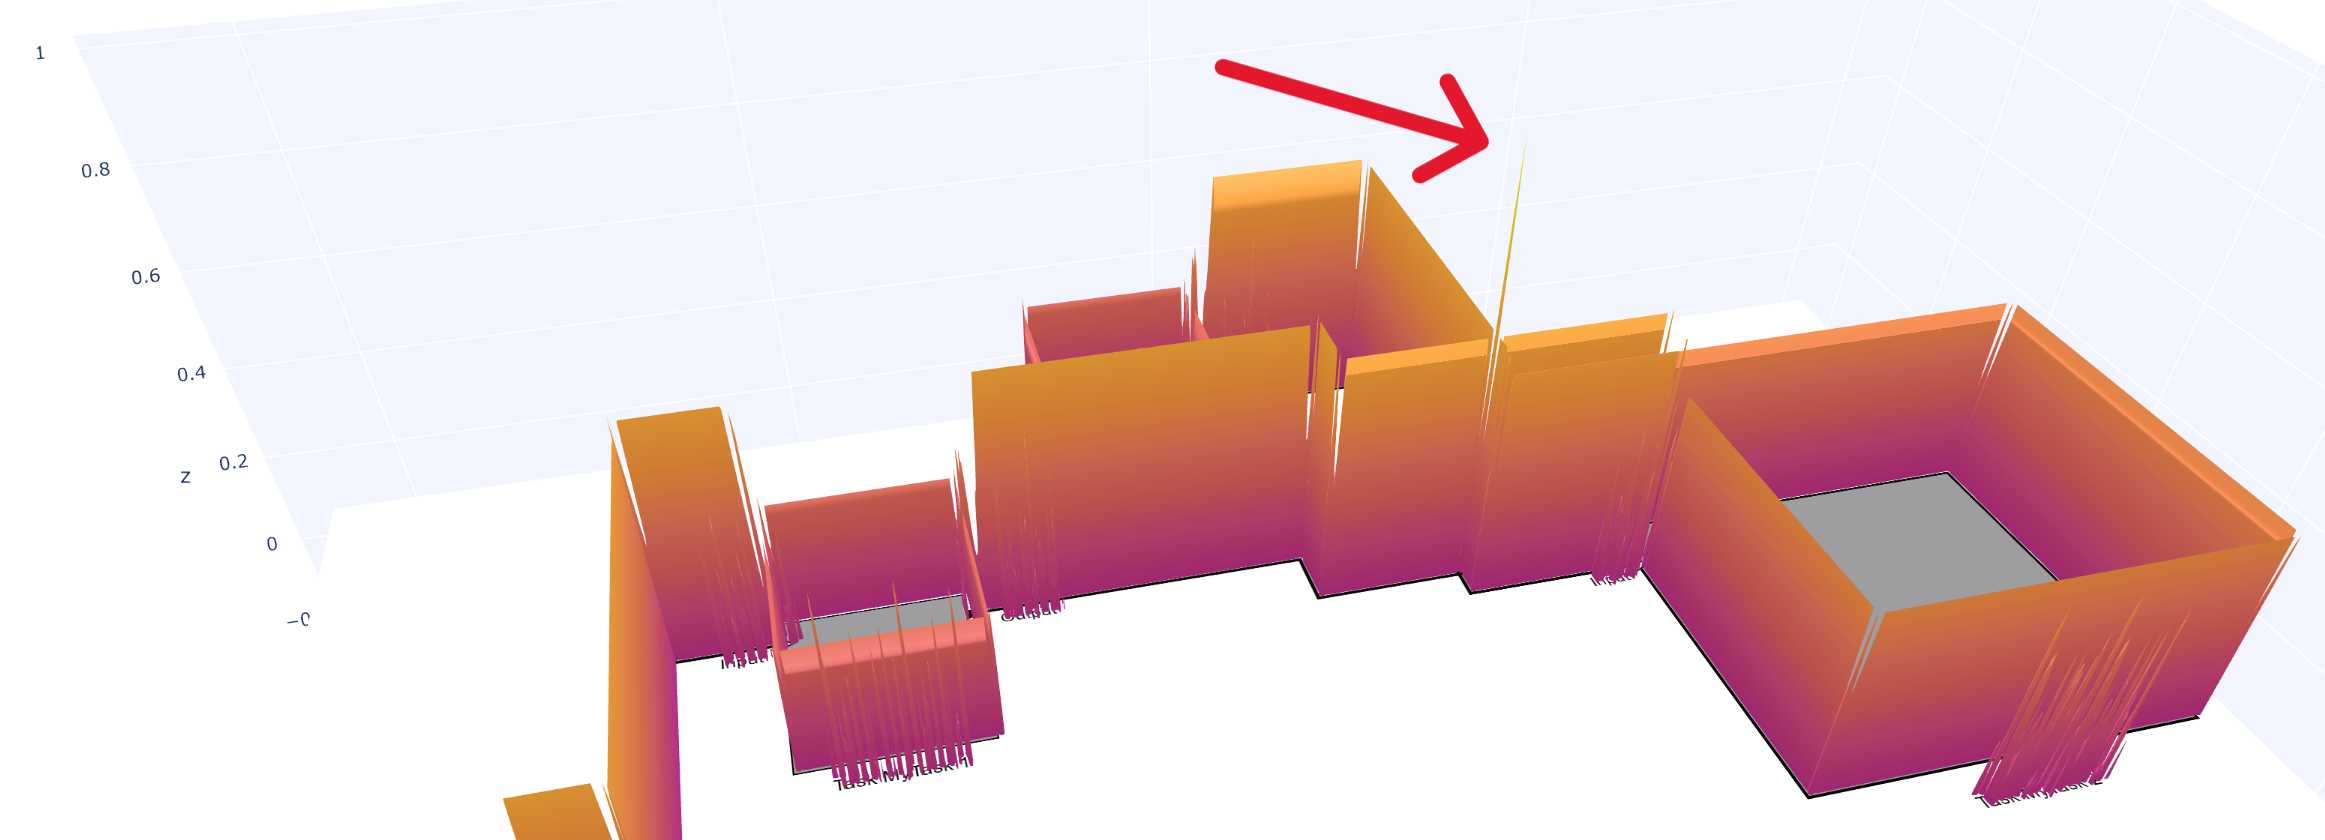
\includegraphics[width=1\linewidth]{pictures/intersection_peak.png}
    \caption{Simmilarity score peaks at an intersection visualized in 3d using \textit{plotly}.}
    \label{fig:intersection_peak}
\end{figure}\\
Misidentified letters and ports are removed by filtering out all line segments with a length shorter than 20 pixels. In all test cases, this approach successfully removes the unwanted line segments while keeping the edges, illustrated in \autoref{fig:comparison_filter}.\\
As shown in \autoref{fig:threshold}, the \textit{filter2D()} function initially does not detect any edges at intersections, leading to gaps between the line segments. To process these gaps, it is assumed that intersections always consist of two straight edges. Overlapping 90\textdegree\ turns are considered impossible and will result in an error caused by the incorrect edge recognition, as it would result in an ambiguous diagram. This forces the user to maintain a clear diagram structure.\\
First, all intersections in the image are detected using \acrshort{opencv}'s \textit{matchTemplate()} function, which matches a template image of an intersection to overlapping regions of the target image \cite{opencv_matchTemplate_2024}.\\
The function slides the template across the image, comparing overlapping patches with the template using a specified method. Among the available methods \cite{opencv_comparison_methods_2024}, \textit{tm\_sqdiff\_normed} produced the most accurate results. For each pixel, the function calculates and assigns a value representing the similarity between the template and the corresponding image region below. While this approach is more precise than \textit{filter2D()}, it is also significantly more resource-intensive.\\

\begin{wrapfigure}{R}{0.4\textwidth}
    \centering
    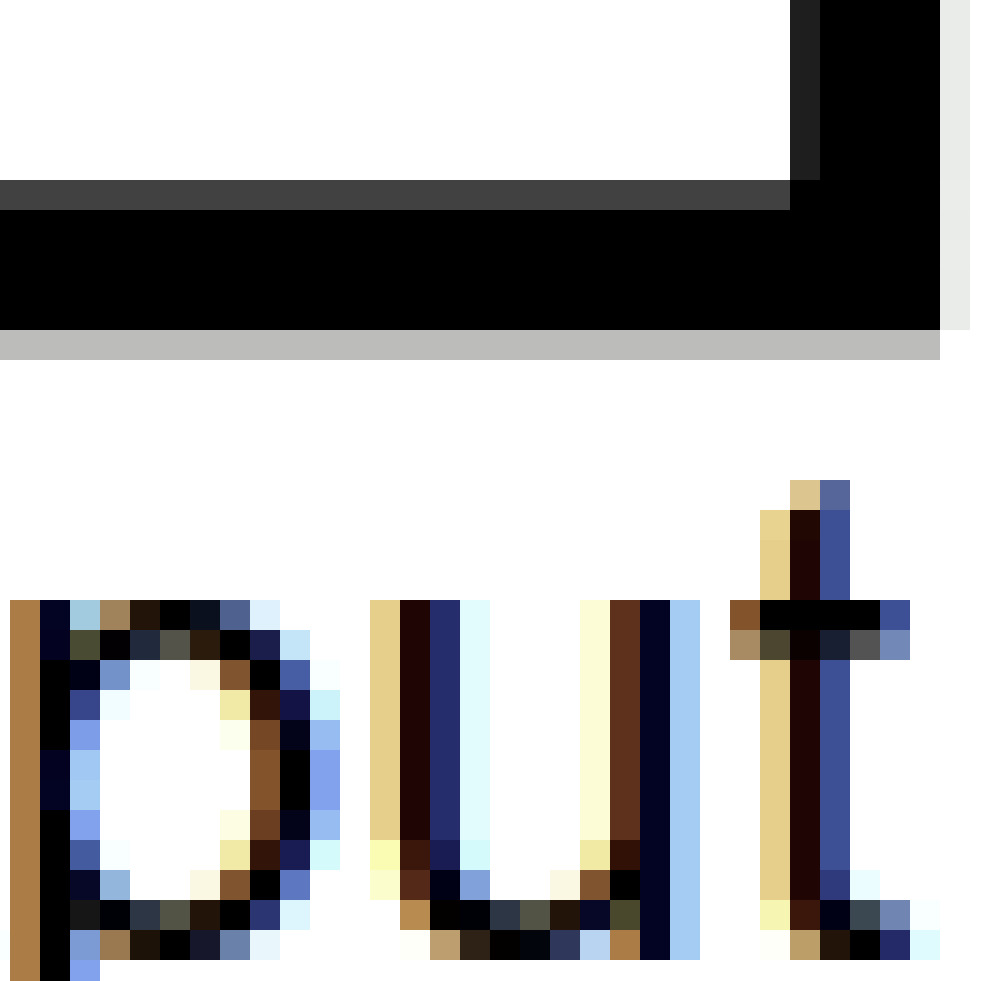
\includegraphics[width=\linewidth]{pictures/aliasing.png}
    \caption{Aliasing typically found near hard edges to increase the apparent resolution or contrast. The shade of gray is not the same on both sides of the edge.}
    \label{fig:aliasing}
\end{wrapfigure}
At intersections, the similarity value is approximately 85$\%$. This slight discrepancy likely arises from how modern operating systems use aliasing to render text and lines with higher apparent resolution and contrast compared to the display. Zooming in reveals that the white pixels near edges and text are often replaced with subtle color hues or shades of gray.\\
Rendering the results of the template matching highlights a peak in similarity at the intersection (\autoref{fig:intersection_peak}). Thresholding isolates this peak, typically yielding two or more matches per intersection. These matches are then filtered based on proximity, ensuring only one match is detected at each intersection.\\
The method then processes each detected intersection by connecting the two vertical and two horizontal line segments adjacent to it. This eliminates any residual points near the intersection, leaving only one vertical and one horizontal line segment, as illustrated in \autoref{fig:intersection_before_after}.\\
In the allocations editor, the same approach is applied to detect and process signal containers on edges.\\
To enhance diagram readability, it is assumed that no 90\textdegree\ turns are concealed behind the containers and that edges pass through them in a straight line, avoiding ambiguities that could confuse both computer vision algorithms and human users. The primary distinction from intersection detection lies in the number of line segments: at a signal container, only two line segments meet, rather than four.

\begin{figure}[ht]
    \centering
    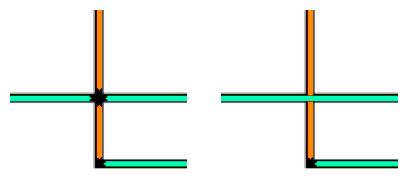
\includegraphics[width=0.7\linewidth]{pictures/intersection_before_after.png}
    \caption{Intersection before and after connecting the line segments.}
    \label{fig:intersection_before_after}
\end{figure}
Converting the line segments into polylines at this stage would produce unusable data, as the segments are not grouped and not sorted in the sequential order of the edge's \textit{flow}. To generate proper polylines, the line segments must first be grouped into multiple lists of connected chains which then have to be sorted into the correct order. For instance, if the first line segment in the list is an intermediate segment within an edge, the polyline function may mistakenly attempt to connect its endpoints directly to the next point in the list, without considering whether it belongs to the same continuous chain, resulting in incorrect edge detections.\\
The implemented method begins by selecting the first line segment, adding it as a starting point to the first chain group and to a list of used segments and setting the \textit{chain\_growing} flag to true. It then iterates through all remaining segments, checking whether each segment has already been used and whether any of its points lie within 7 pixels of the points of the current segment. If a match is found, the segment is added to the \textit{used\_segments} list and the current chain group. If no segment is found within the 7-pixel threshold, the \textit{chain\_growing} flag is set to false, and the completed chain group is added to the list of chains. A threshold of 7 pixels was selected as it reliably produces connected polylines while ensuring that closely positioned lines, such as those at ports, remain distinct and separate. This process continues until all line segments have been assigned to a group as in \autoref{fig:chains_before_after}.
\begin{figure}[ht]
    \centering
    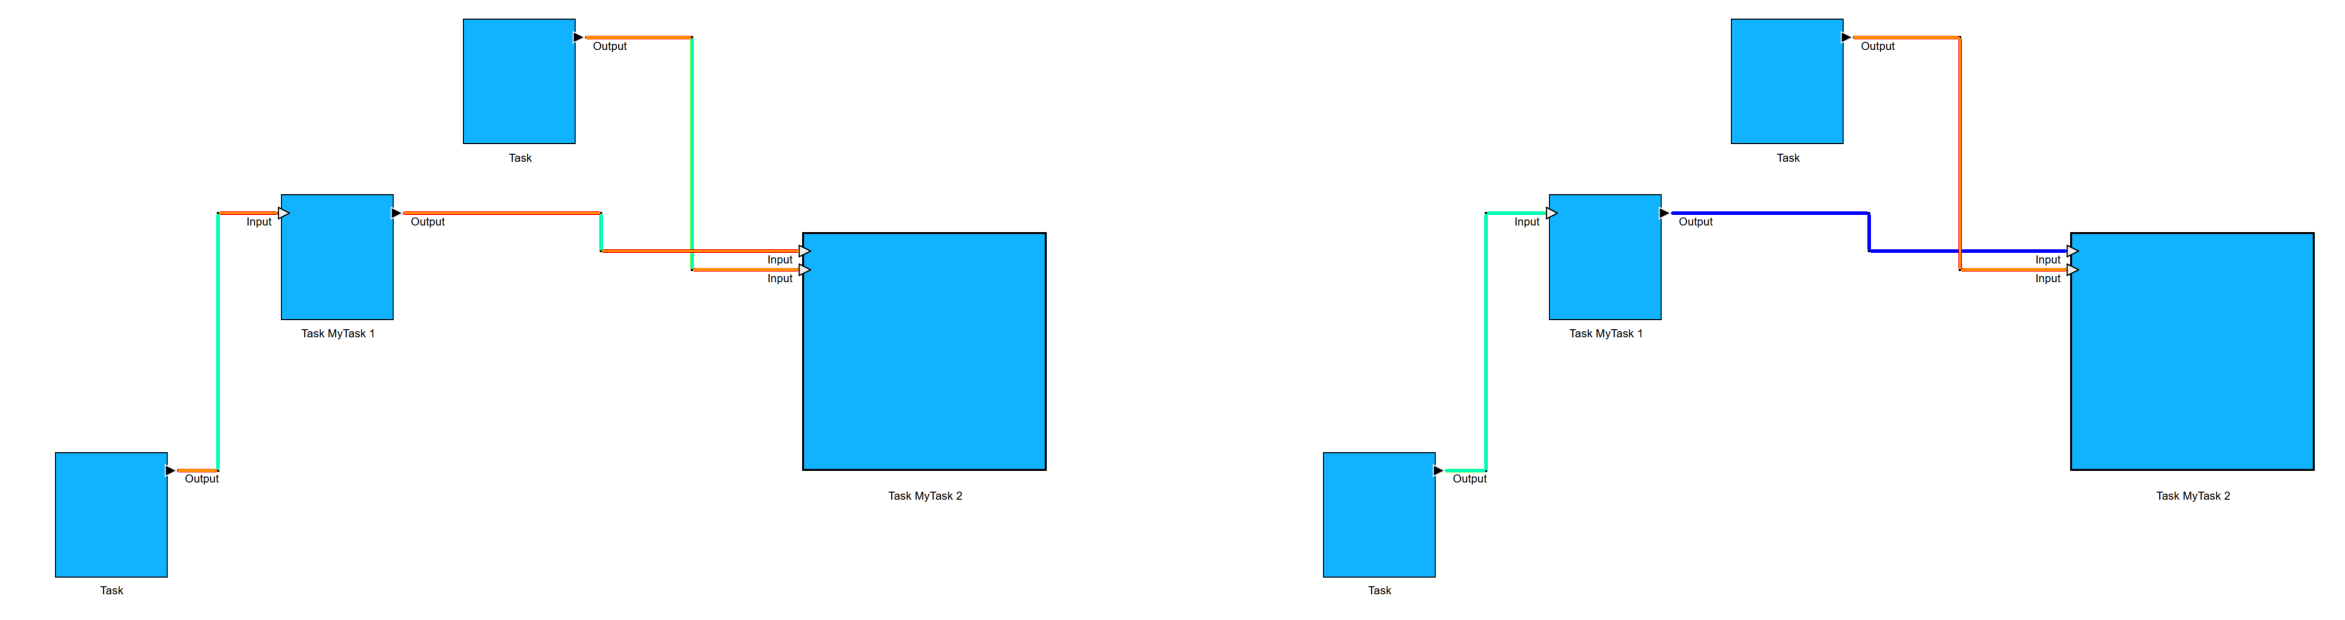
\includegraphics[width=\linewidth]{pictures/chains_before_after.png}
    \caption{Left: detected vertical and horizontal line segments\\Right: detected line segments grouped into colored line segment chains} % TODO: switch blue and orange colors to be consistent with other figures
    \label{fig:chains_before_after}
\end{figure}\\
Generating the polylines now would yield better results, but still create unusable data, because the line segments within each chain and the two points within each line segment are not sorted. The first point in a list of line segments in a chain could for example be a point in the middle of the chain, resulting in \acrshort{opencv}'s Polyline function to connect the following points in the wrong order.\\
The sorting algorithm for solving this problem consists of two steps: the first sorts the line segments from the beginning of the chain to the end, the second sorts the end- and startpoint of each line segment individually, so that they too appear in sequential order of 'flow' in the chain.\\
To distinguish between intermediate points and endpoints, the function relies on the method by which the points were initially identified: when two line segments intersect to form a 90\textdegree\ turn, each segment consists of a start- and an endpoint. As a result, intermediate points in a chain, where line segments meet, always have two points in close proximity, whereas endpoints only have a single point, since only one line segment terminates at each endpoint (see \autoref{fig:point_zoom}).
The function leverages this discrepancy by identifying endpoints through an iterative process: It examines each point and checks for the presence of other points within a seven-pixel radius. If no other points are found within this radius, the point is classified as an endpoint of a chain.\\
\begin{figure}
    \centering
    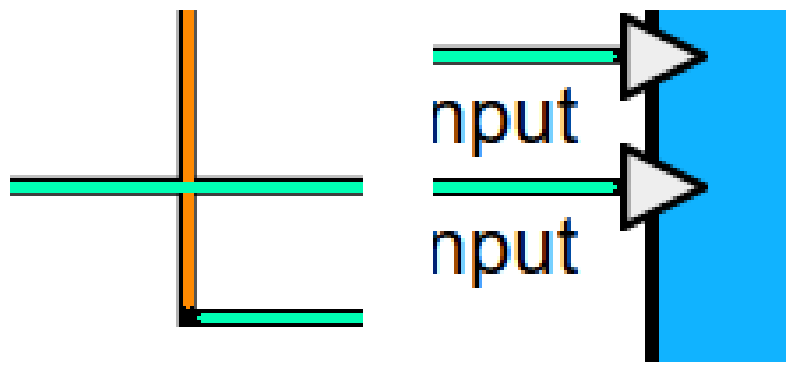
\includegraphics[width=0.5\linewidth]{pictures/zoomed_in_points.png}
    \caption{Intermediate points (left) have other points in close proximity, while endpoints (right) do not.}
    \label{fig:point_zoom}
\end{figure}
Using the identified endpoints to initialize the \textit{sorted\_chain} list allows the program to organize the chains systematically. The process begins by selecting a segment that includes one of the start points as the initial segment of the chain. The endpoint of this segment that is not a chain endpoint is designated as the first \textit{last\_point} in the \textit{sorted\_chain} list. To determine the next segment in the chain, a \textit{lambda function} iterates through each remaining segment in the current chain, calculating the distance between the \textit{last\_point} and each point of each segment in the chain. The segment containing the point with the smallest distance to the \textit{last\_point} is selected as \textit{next\_segment} and removed from the list of \textit{remaining\_segments}. Within this segment, the point closest to the \textit{last\_point} is appended first to the \textit{sorted\_chain}, followed by the second point of the segment. This process repeats until no segments remain in the \textit{remaining\_segments} list. The entire process is repeated for each chain until all points in all chains are ordered according to the edge's \textit{flow}.

Polylines, which represent connected line segments as ordered lists of points, are a fundamental component in reconstructing edges within the diagram. To generate these polylines from the sorted chains, the method iterates through the \textit{sorted\_chains} list, sequentially appending each point to construct the polylines. The preprocessing and sorting of the data ensures that the chains are already structured correctly, making the generation of polylines straightforward and efficient. Once the polyline is constructed, it is converted into the format required by \acrshort{opencv} for further processing.

\section{Vertex Detection}
\label{sec:vertex_detection}
Vertices represent distinct visual elements within \acrshort{xgee}, such as functions, devices, containers or \acrshort{io} ports. Identifying these vertices is critical for interpreting the structural arrangement of the diagrams. This section introduces a template-matching approach to address problems including overlapping vertices and varying sizes, ensuring a more reliable vertex detection in all relevant diagram types within \acrshort{xgee}.

A major problem in template matching is the diversity of vertices within \acrshort{xgee}'s three editor models. For example, the functions editor contains only functions, inputs and outputs, while the hardware editor contains devices and \acrshort{io} ports and the allocations editor contains devices, signal containers, signal arrows and subtasks which overlap with devices and contain their own set of \textit{sub-sub-vertices}. Additionally, some vertices are scalable, while others are not. Scalable vertices require extra processing to ensure accurate detection. However, applying this processing universally to all vertices would result in unpredictable and incorrect detections.

To address these challenges, the model is queried for a list of unique vertices. This list is analyzed to identify any vertices with the \textit{isSubVertexBody}-flag set, which indicates they are subvertices such as subtasks, that overlap with other vertices. These subvertices are prioritized and placed at the beginning of the list of vertices. This way, the vertex detection method can progressively simplify the image by erasing detected subvertices after the first iteration of the vertex detection function, allowing the underlying vertices to be detected without obstruction. Other relevant flags are:
\begin{itemize}
    \item \textit{isScalable} which indicates whether the vertex can be scaled
    \item \textit{sizeX} and \textit{sizeY} which specify the size of the vertex
    \item \textit{filepath} which specifies the path to the template image
    \item \textit{parent\_filepath} which specifies the path to the parent vertex in case it is a subvertex
\end{itemize}
The method iterates through the list of unique vertices in the current editor model, prioritizing subvertices identified in the previous step. These subvertices are removed from the image by setting all pixels within the bounding box of the subvertex to the \textit{fill} color of the parent vertex as shown in \autoref{fig:draw_boxes}. This process effectively removes the subvertices from the image, enabling the subsequent vertex detection steps to accurately identify the remaining vertices.\\
\begin{figure}[htb]
    \centering
    \begin{minipage}[b]{0.45\textwidth}
        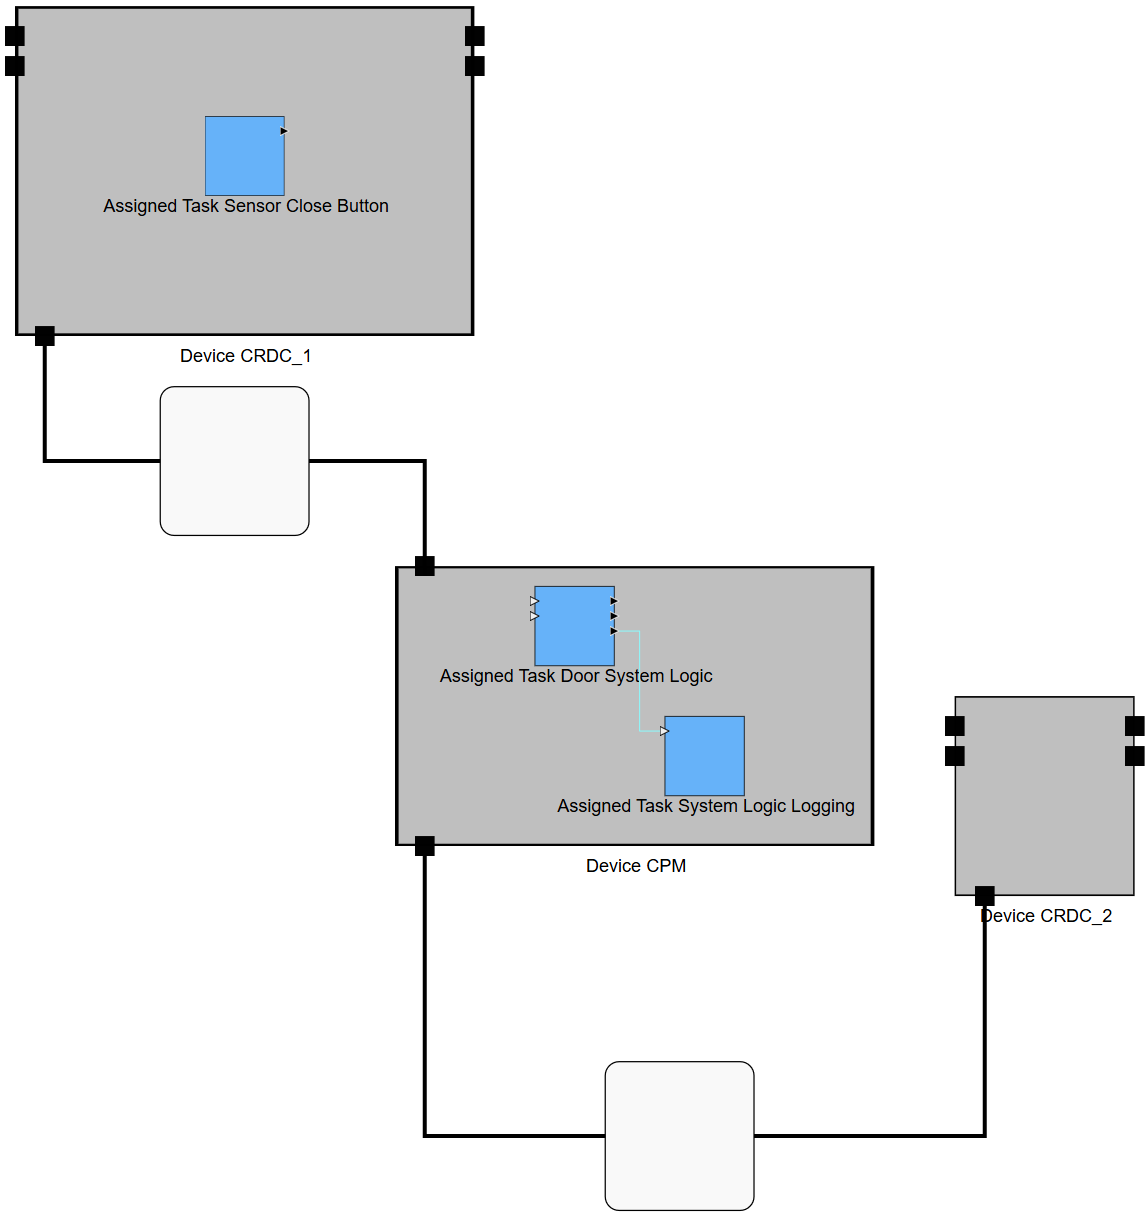
\includegraphics[width=\textwidth]{pictures/draw_boxes_before.png}
    \end{minipage}
    \hfill
    \begin{minipage}[b]{0.45\textwidth}
        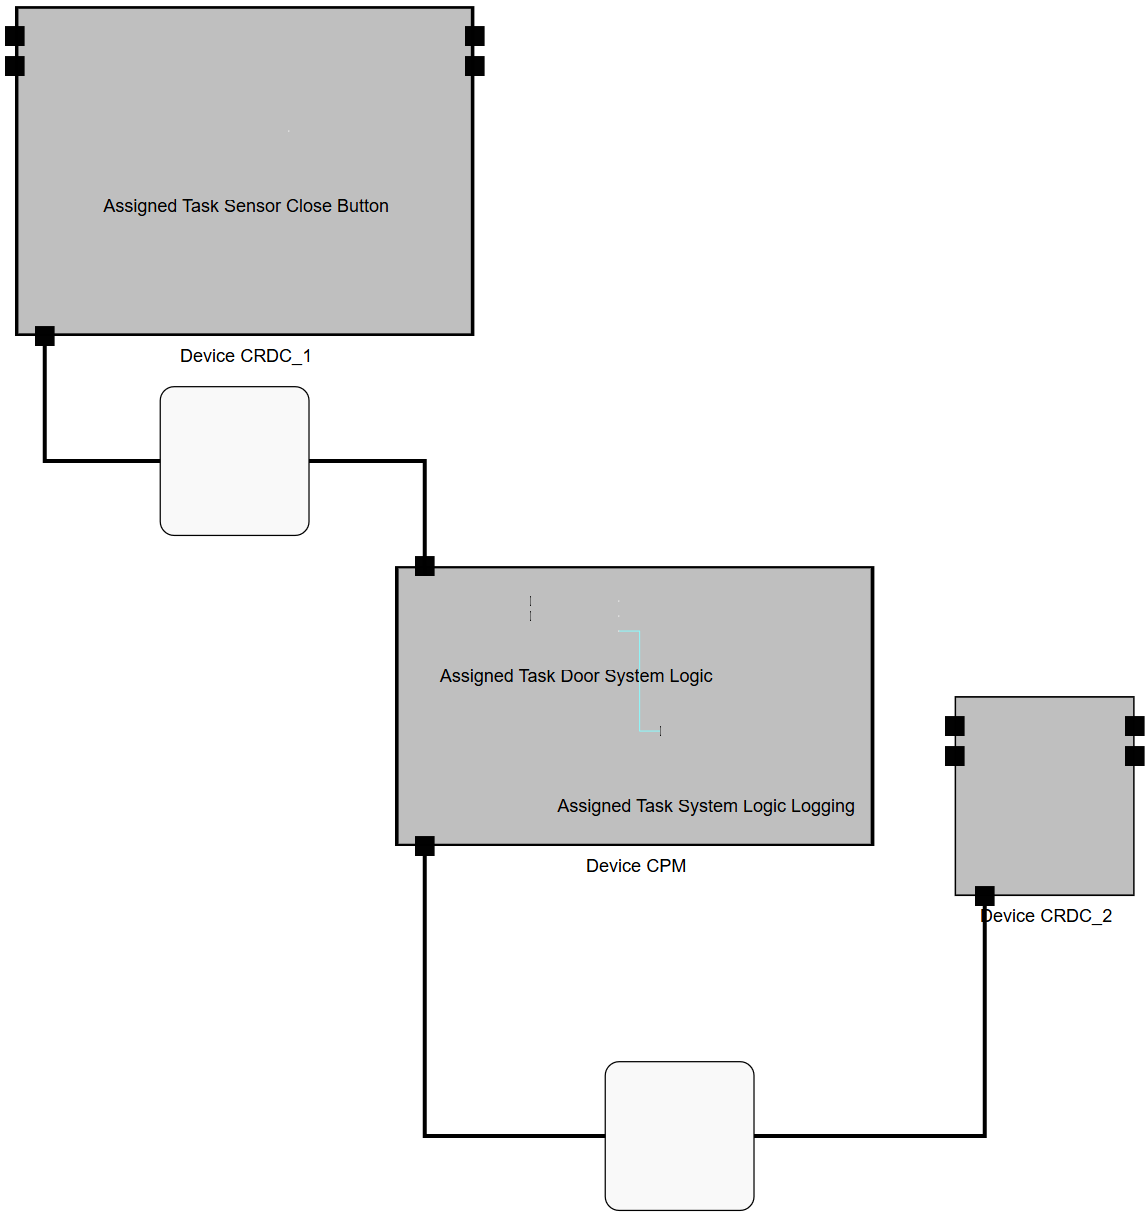
\includegraphics[width=\textwidth]{pictures/draw_boxes_after.png}
    \end{minipage}
    \caption{Original image from allocations editor containing subvertices (left) and modified image with subvertices removed (right).}
    \label{fig:draw_boxes}
\end{figure}
After processing the subvertices, a new image wrapper object is created using the modified image. The method then iterates through the list of remaining vertices, loading the template image of each vertex using the \textit{filepath} attribute. Depending on the \textit{isScalable} flag, an object of either the \textit{ScalableVertexDetector} or \textit{PortDetector} class is created and the corresponding vertex detection is applied.\\
In case of unscalable vertices, \acrshort{opencv}'s \textit{matchTemplate} and \textit{normalize} functions are applied. The resulting data is thresholded to identify the positions of all found vertices. To define the vertex boundaries, the \textit{sizeX} and \textit{sizeY} attributes are used, allowing bounding boxes of the correct size to be drawn with the detected match serving as the upper-left corner. This approach is effective for detecting vertices like \acrshort{io} ports and subtasks.\\
In case of scalable vertices, this approach does not work because the size of the vertex is variable, which reduces the certainty of found matches drastically and eliminates constant \textit{sizeX} and \textit{sizeY} values as a reliable method for defining bounding boxes.\\

Scalable vertices within \acrshort{xgee} are function and device containers that can be resized to improve the readability of visualizations. However, the initial scalable vertex detection algorithm often produced inaccurate results when applied to large function and device containers. Specifically, it tended to produce higher similarity scores at the corners of the container, as the black border surrounding the vertex at these locations more closely resembled the black border in the template image. In contrast, the absence of a black border in the center of the container led to lower similarity scores. In extreme cases, this resulted in the center of the vertex not being detected at all, with the algorithm instead falsely identifying four smaller vertices at the container's corners. The same issue occurred with large devices.\\
To detect these vertices regardless of their dimensions, multiple templates of the same size for different parts of the large vertex as illustrated in \autoref{fig:templates} are required. They are generated from the (leftmost) original template image by cropping its edges and corners in different ways.
\begin{figure}[ht]
    \centering
    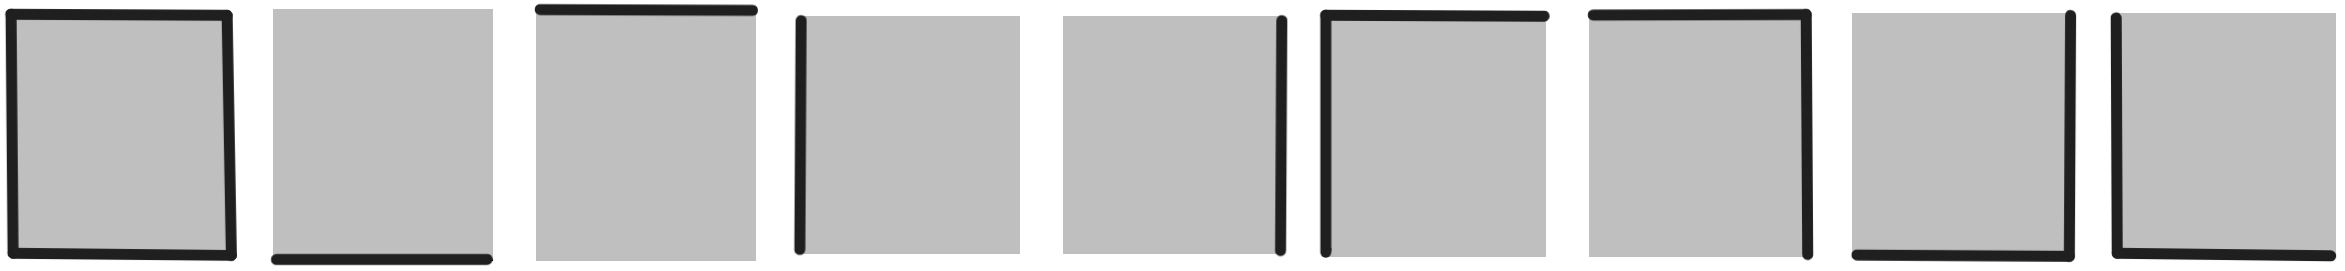
\includegraphics[width=0.85\linewidth]{pictures/templates.png}
    \caption{Templates for scalable vertex detection generated from the original (leftmost) template image, black edges are exagerated for better visibility.}
    \label{fig:templates}
\end{figure}
Template matching is performed iteratively with each template, comparing the results after each iteration. The highest similarity score for each pixel is retained and combined into the resulting data, which is then thresholded to extract all potential matches.\\
Typically, numerous matches are identified during this process. To eliminate false positives and process the matches to determine the differently sized bounding boxes of the vertices, the algorithm described by Andreas Waldvogel and Bj{\"o}rn Annigh{\"o}fer in \cite{waldvogel_annighoefer_models_2024} is applied.\\
The original image is thresholded to distinguish foreground from background pixels, as illustrated in \autoref{fig:foreground_threshold}. This foreground information is then utilized to filter the detected matches, retaining only those located within the foreground area. This process effectively removes false positives which often occur because the black pixels along the edges and borders of function or device containers closely resemble those in the black borders in the template images.
\begin{figure}[htb]
    \centering
    \begin{minipage}[b]{0.36\textwidth}
        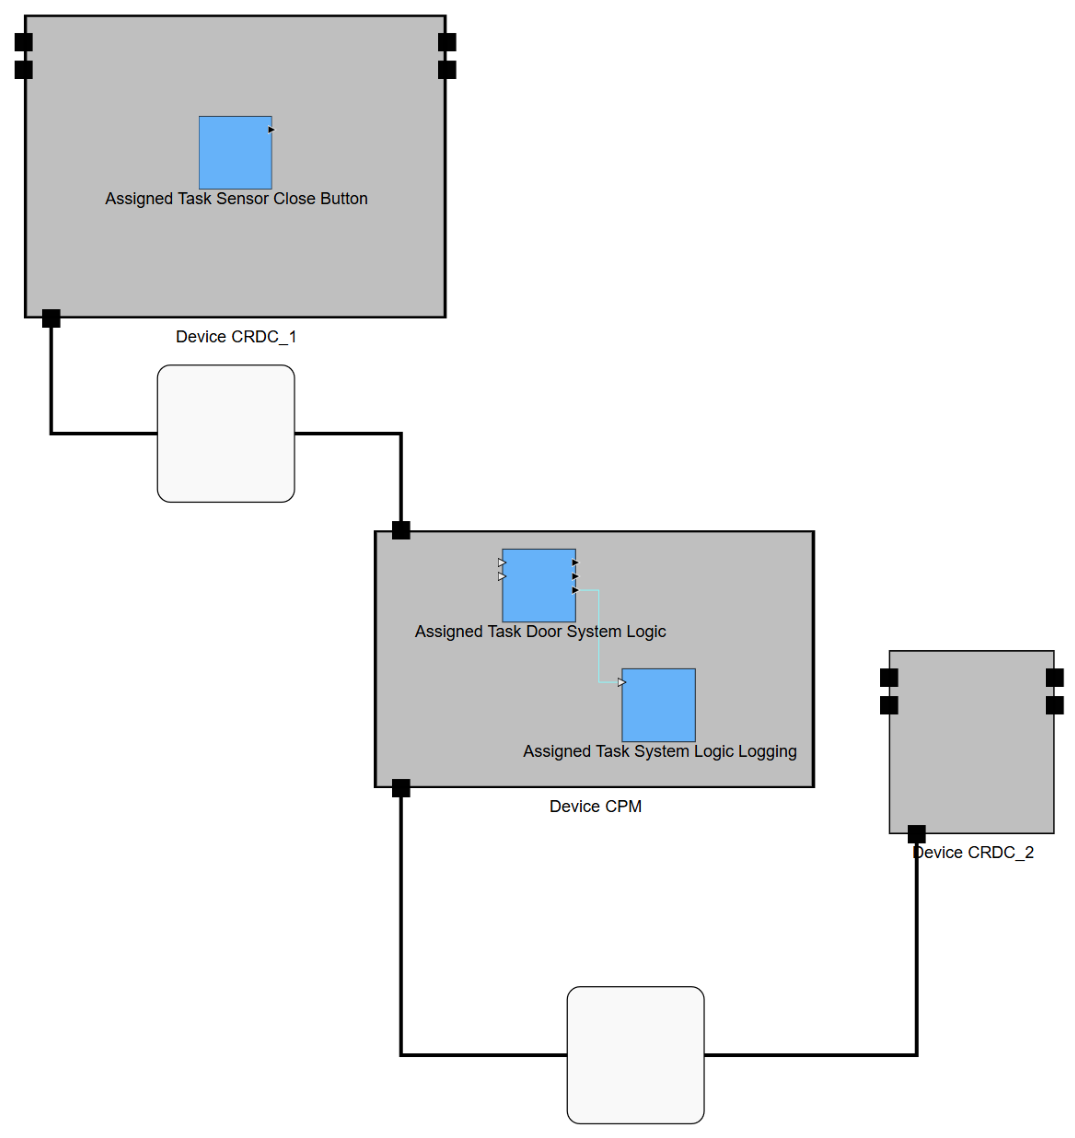
\includegraphics[width=\textwidth]{pictures/foreground_threshold_before.png}
    \end{minipage}
    \hfill
    \begin{minipage}[b]{0.36\textwidth}
        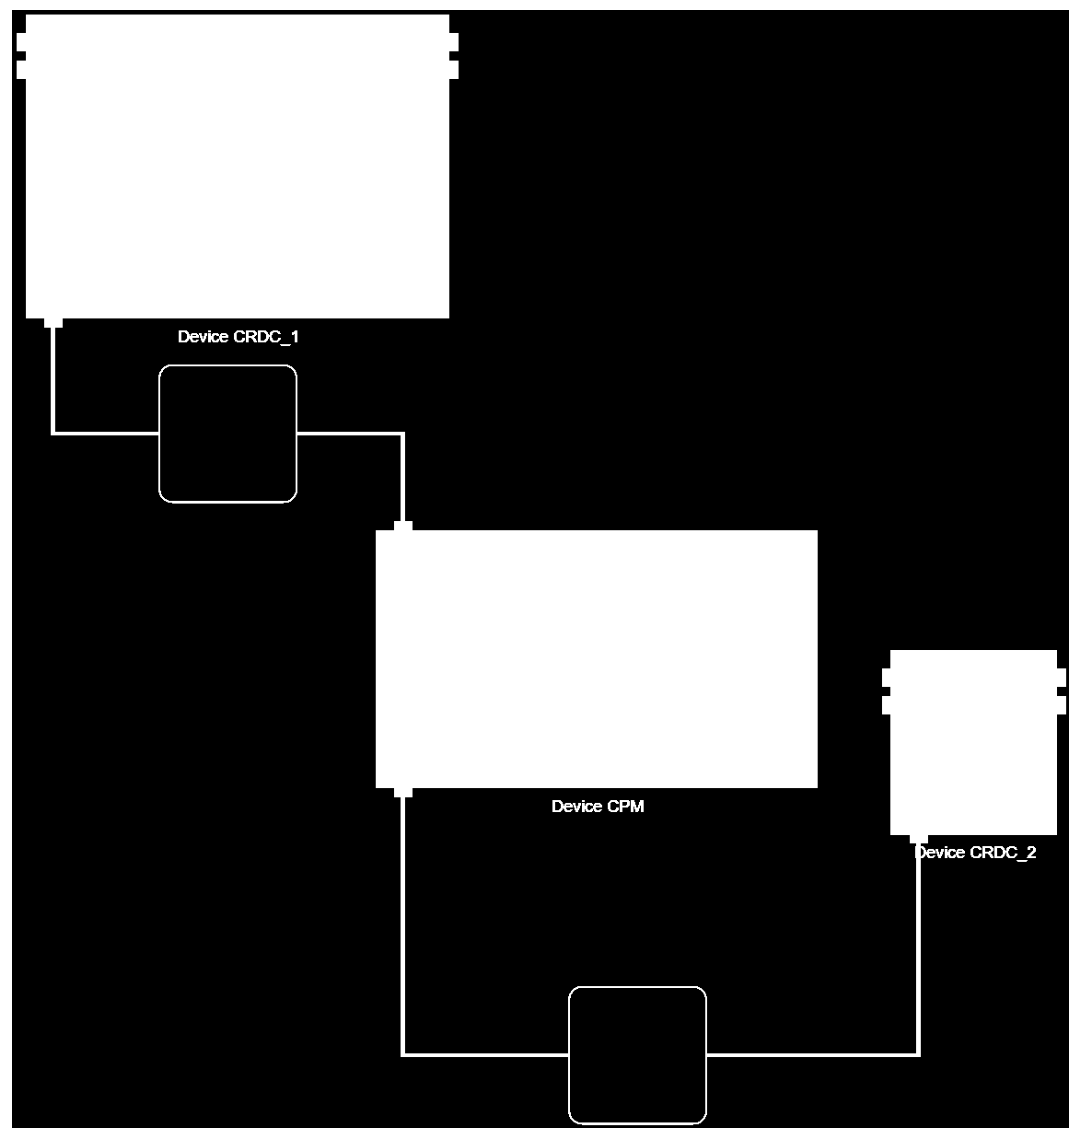
\includegraphics[width=\textwidth]{pictures/foreground_threshold_after.png}
    \end{minipage}
    \caption{The allocations editor screenshot (left) is thresholded to extract the foreground pixels (right).}
    \label{fig:foreground_threshold}
\end{figure}\\
For each remaining detected match, the \textit{sizeX} and \textit{sizeY} attributes are used to create a filled bounding box around the detected position. Since multiple matches are often found at various locations within a single large vertex, the overlapping bounding boxes collectively form a larger structure. This structure is then simplified into a single bounding box using \acrshort{opencv}'s \textit{findContours} function.
\begin{figure}[htb]
    \centering
    \begin{minipage}[b]{0.36\textwidth}
        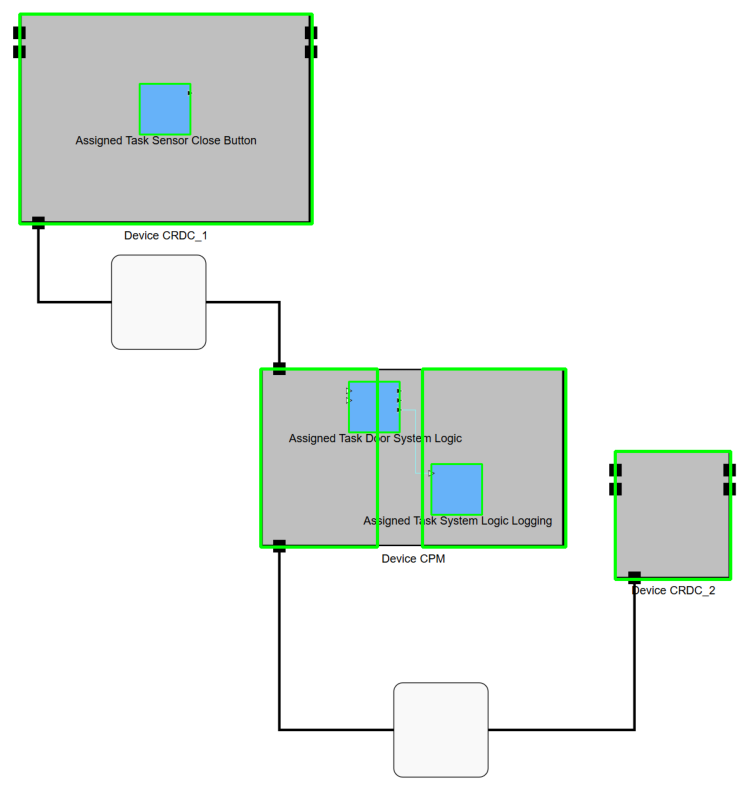
\includegraphics[width=\textwidth]{pictures/many_templates_before.png}
    \end{minipage}
    \hfill
    \begin{minipage}[b]{0.36\textwidth}
        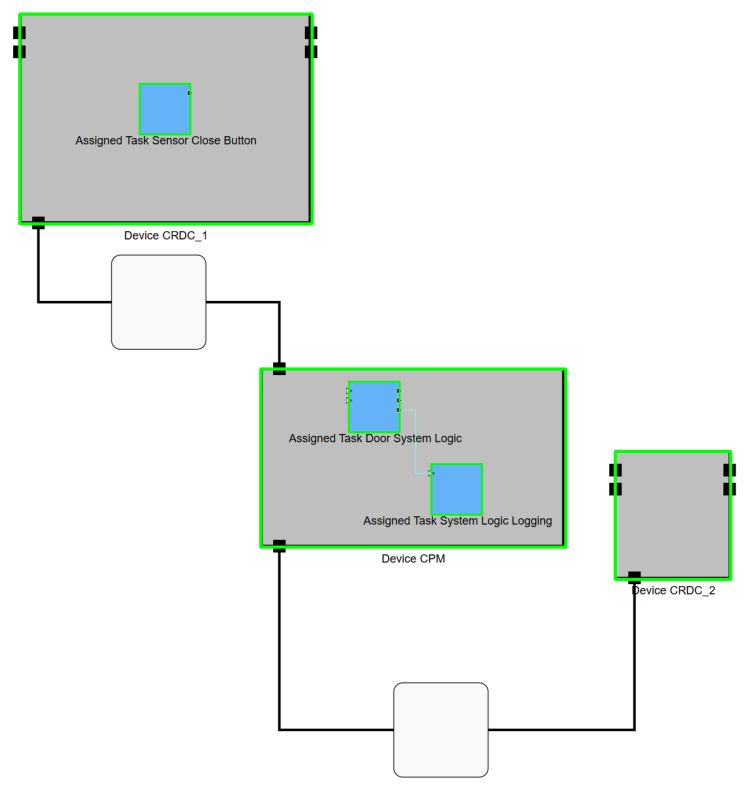
\includegraphics[width=\textwidth]{pictures/many_templates_after.png}
    \end{minipage}
    \caption{Image from allocations editor containing a large, partially detected device using one template(left) and containing a large, fully detected device using multiple templates(right).}
    \label{fig:many_templates}
\end{figure}
This approach successfully detects all scalable vertices within \acrshort{xgee}, regardless of their dimensions. Using both scalable and non-scalable vertex detection methods ensures that all vertices are detected accurately, regardless of their size or complexity.\\
The method is capable of detecting all vertices in the 20 unique test cases within this paper, including subvertices and scalable vertices.

\section{Text Recognition}
\label{sec:text_recognition}
The original text detection in \acrshort{xgee} utilized Pytesseract \ref{pytesseract_2024}, an open-source \acrlong{ocr} (\acrshort{ocr}) engine developed and sponsored by Google in 2006. Pytesseract required separate installation from other packages and could only detect text in images that had been preprocessed. Additionally, the output data required extensive postprocessing to become usable. While Pytesseract demonstrated high accuracy and speed, it struggled to reliably detect small text or text with low contrast to the background. Its optimization for structured text formats, such as those found in books, further hindered its performance in \acrshort{xgee}, where text can appear in varying orientations, sizes, and positions. These limitations made reliable text detection using Pytesseract difficult to achieve.

After evaluating various \acrshort{ocr} engines, including Easy\acrshort{ocr} \cite{easyocr_2024}, Doctr \cite{doctr_2024}, and Keras-\acrshort{ocr} \cite{keras_ocr_2023}, Easy\acrshort{ocr} proved to be the most suitable alternative.\\
Easy\acrshort{ocr} is a deep-learning-based \acrshort{ocr} engine that reliably detects text in images, even under challenging conditions such as low contrast or resolution. Although it operates more slowly on modern \acrshort{cpu}s compared to some alternatives, it performs significantly faster on \acrshort{gpu}s. Additionally, its ability to detect text in multiple languages adds potential value for future applications. Integration of Easy\acrshort{ocr} into the \acrshort{xgee} editor for the user is straightforward, as it can be installed directly via pip install easy\acrshort{ocr} through the requirements.txt file without requiring additional dependencies or downloads. Unlike Pytesseract, Easy\acrshort{ocr} only necessitates minimal image preprocessing, and it structures found characters into words and sentences automatically based on proximity, eliminating the need for extensive postprocessing. These advantages make Easy\acrshort{ocr} the optimal choice for the updated text detection pipeline within \acrshort{xgee}.

\begin{figure}[htb]
    \centering
    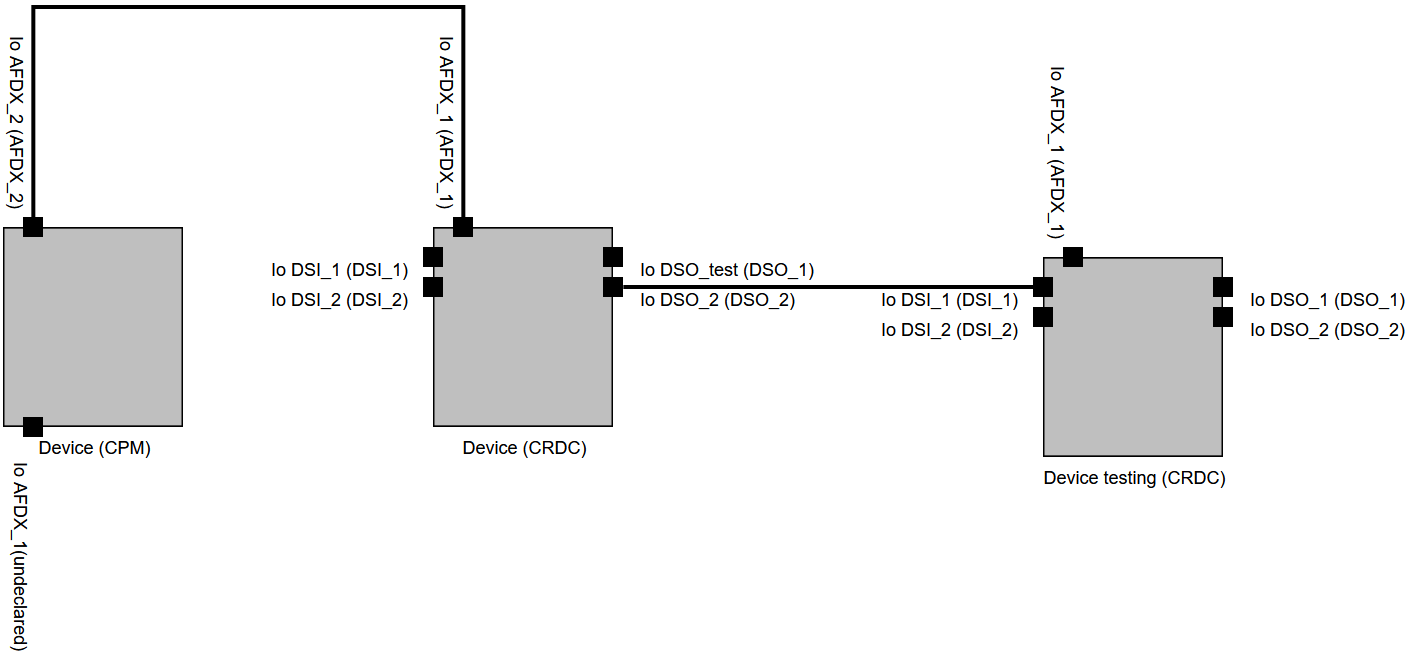
\includegraphics[width=0.8\linewidth]{pictures/text_before.png}
    \caption{Input image from function editor containing rotated text}
    \label{fig:text_before}

    \centering
    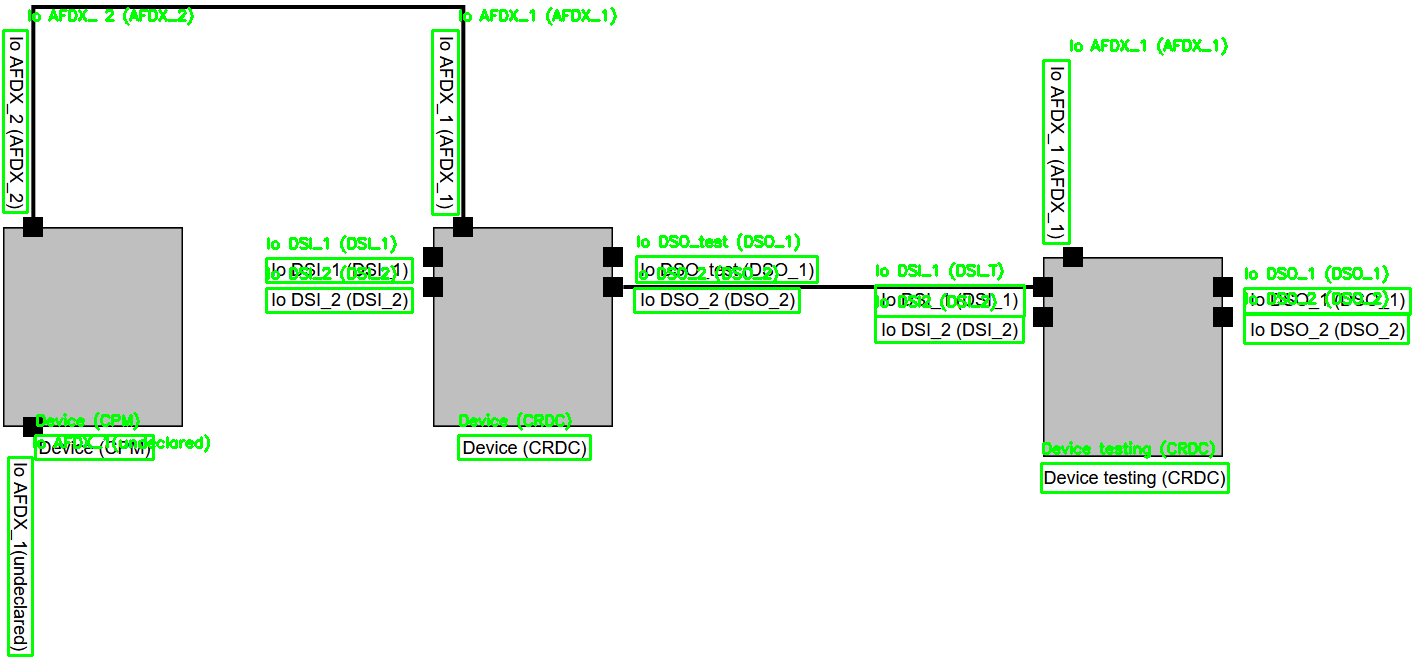
\includegraphics[width=0.8\linewidth]{pictures/text_after.png}
    \caption{Output image from function editor containing text bounding boxes}
    \label{fig:text_after}
\end{figure}
First, a reader object is created and the language of the text is specified. The readtext function of the reader object is then called with the image as an argument. The image has to be padded to have a square shape, so it can be easily rotated. To ensure a more reliable detection, the image is slightly blurred and upscaled to counter any aliasing and small characters. The text detection function then returns a list containing the detected text, its bounding box, and a certainty factor. Parameters can be specified when calling this function to adjust the expected text properties, enhancing the reliability of the detection. For example in earlier versions, Easy\acrshort{ocr} struggled to detect single characters, but with these parameter adjustments, this issue has been mostly resolved. The detection process is repeated for the rotated version of the image to detect rotated text labels, present in the hardware layer, as well. The positions of the bounding boxes of the found rotated text are then rotated around the center of the image to reallign them with the found text of the original image. The found bounding boxes and text are illustrated in \autoref{fig:text_before} and \ref{fig:text_after}. Reading an image which contains rotated text usually results in many falsely read characters, because for example 'o' and 'l' can be interpreted regardless of orientation. To filter out the falsely read characters, the algorithm first combines the found results of both \acrshort{ocr}-searches and then removes every word shorter than three letters.\\

Because easy\acrshort{ocr} automatically groups detected characters into words and sentences, this is a simple and effective method to filter out falsely read characters. Using this approach also allows the same algorithm to be used for all models, regardless of the \acrshort{xgee} editor they were created in, simplifying the integration into the \acrshort{xgee} codebase.